\subsection{rfmodel Struct Reference}
\label{structrfmodel}\index{rfmodel@{rfmodel}}
{\tt \#include $<$bpm\_\-interface.h$>$}

Collaboration diagram for rfmodel:\nopagebreak
\begin{figure}[H]
\begin{center}
\leavevmode
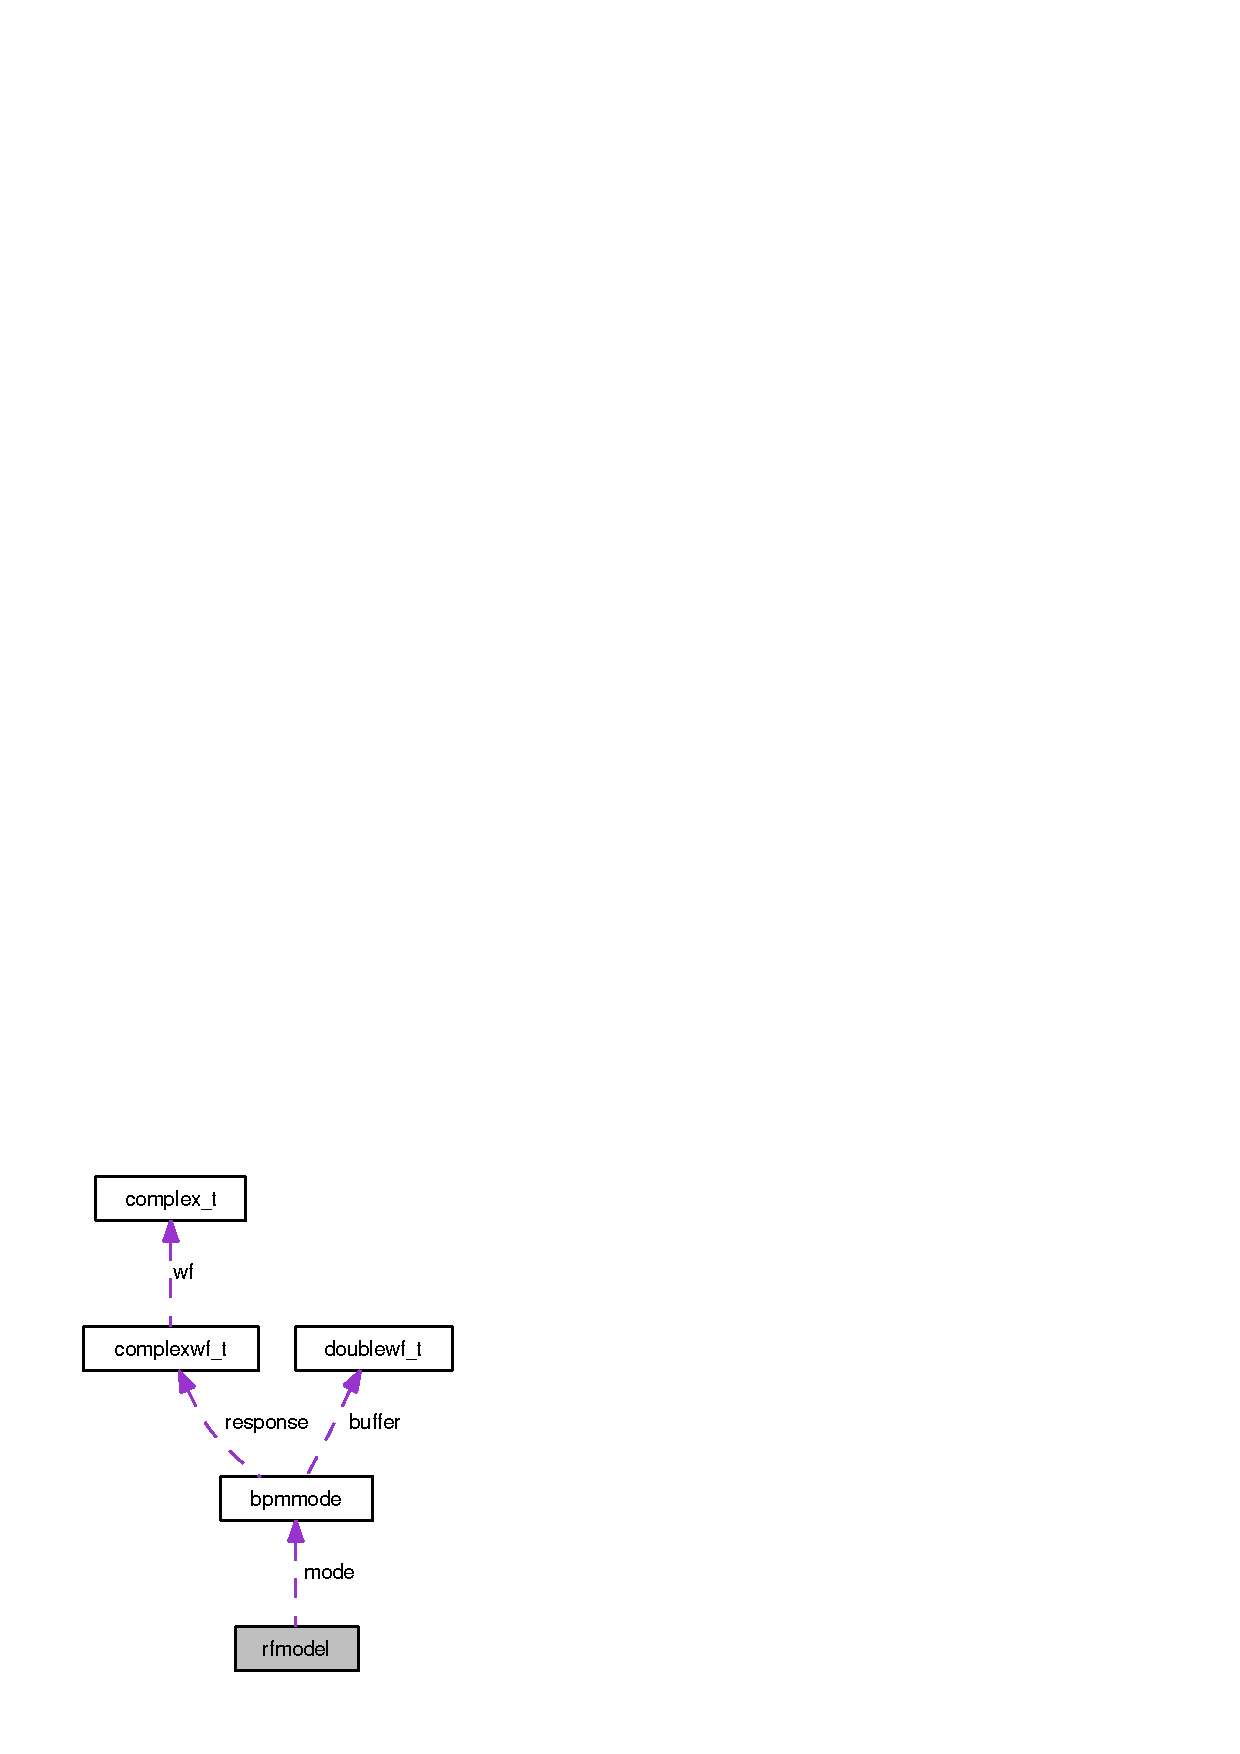
\includegraphics[width=110pt]{structrfmodel__coll__graph}
\end{center}
\end{figure}


\subsubsection{Detailed Description}
This structure contains the complete RF model for a BPM, which is essentially a collection of it's resonant modes and sensitivities 

Definition at line 296 of file bpm\_\-interface.h.\subsubsection*{Data Fields}
\begin{CompactItemize}
\item 
char {\bf name} [20]
\item 
int {\bf nmodes}
\item 
{\bf bpmmode\_\-t} $\ast$ {\bf mode}
\end{CompactItemize}


\subsubsection{Field Documentation}
\index{rfmodel@{rfmodel}!name@{name}}
\index{name@{name}!rfmodel@{rfmodel}}
\paragraph[name]{\setlength{\rightskip}{0pt plus 5cm}char {\bf rfmodel::name}[20]}\hfill\label{structrfmodel_0347645ae53fe9060133b86a13dff957}


A name for the cavity's RF model 

Definition at line 297 of file bpm\_\-interface.h.\index{rfmodel@{rfmodel}!nmodes@{nmodes}}
\index{nmodes@{nmodes}!rfmodel@{rfmodel}}
\paragraph[nmodes]{\setlength{\rightskip}{0pt plus 5cm}int {\bf rfmodel::nmodes}}\hfill\label{structrfmodel_d540be1e4090f1a5f0473ef98924422d}


The number of BPM modes in the model 

Definition at line 298 of file bpm\_\-interface.h.\index{rfmodel@{rfmodel}!mode@{mode}}
\index{mode@{mode}!rfmodel@{rfmodel}}
\paragraph[mode]{\setlength{\rightskip}{0pt plus 5cm}{\bf bpmmode\_\-t}$\ast$ {\bf rfmodel::mode}}\hfill\label{structrfmodel_b4dbc2c56b212e42858185090cfdd0ac}


A list of pointers to the array of modes 

Definition at line 299 of file bpm\_\-interface.h.

The documentation for this struct was generated from the following file:\begin{CompactItemize}
\item 
bpminterface/{\bf bpm\_\-interface.h}\end{CompactItemize}
